%----------------------------------------------------------------------------
\chapter{Background} \label{chapter_background}
%----------------------------------------------------------------------------
This chapter introduces the concepts necessary to understand the requirements and ideas behind the rest of the work. In Section \ref{section_background_MDSD}, we take a look at the applicability of modeling in the design of safety-critical reactive systems, followed by the corresponding formal verification techniques in Section \ref{section_background_FORM}. Then, in Section \ref{section_background_behaviorModeling}, a short introduction is given on behavioral modeling, leading to the precise definition of the statechart formalism in  Section \ref{section_background_statechart}, which is commonly used to represent behavioral models and which is a core element of the Gamma Framework. After that, in Section \ref{section_background_comparison}, we examine the action languages of existing tools with respect to their expressive power and possibilities of formal verification. Lastly, in Section \ref{section_background_target} a brief introduction of the Gamma and Theta frameworks is given, which are the target environments of the action language described in the following chapters. 

%----------------------------------------------------------------------------
\section{Model-driven software development} \label{section_background_MDSD}
%----------------------------------------------------------------------------
Due to the application of the modeling concept in several completely different domains, first of all, we need to define the meaning of \textit{model} in this work.
\begin{definition}[Model]
	A model is the simplified image of an element of the real or a hypothetical world (the system), that replaces the the system in certain considerations.
\end{definition}

For a model to be interpretable, executable or formally verifiable, it must be described according to predefined rules in the given domain. This set of rules is provided by \textit{modeling languages}.
\begin{definition}[Modeling Language]
	A modeling language consists of the following elements:
	\begin{itemize}
		\item \emph{Metamodel:} a model defining the building blocks of the modeling language as well
		as their relationships.
		\item \emph{Concrete syntax:} a set of rules defining a graphical or textual notation for the
		element and connection types defined in the metamodel.
		\item \emph{Well-formedness constraints:} a set of constraints that models have to meet in order
		to be deemed valid in the modeling language.
		\item \emph{Semantics:} a set of rules that define the meaning of the element and connection
		types defined in the metamodel. Semantics can be either \textit{operational} (what should happen during execution) or \textit{denotational} (given by translating concepts in a modeling language to another modeling language with well-defined semantics).
	\end{itemize}
\end{definition}

Models can grasp various aspects of a system. Structural models describe the structure of the system, representing knowledge regarding the parts of the system and the properties and connections of these parts. This means that the model describes static knowledge and not temporal change. On the other hand, behavioral models describe the change of the system over time through its changing of states and execution of processes. These categories do not cover every aspect of a system, and usually cannot be separated this well in practical applications. For instance, action languages of state-based models describe the behavior of the system in a procedural way. There are several possible formalisms for both kinds of models, some of which are discussed in Section \ref{section_background_behaviorModeling}.

Model-driven software development (MDSD) is a software development methodology that utilizes domain models as the primary artifact throughout the entire software development process. This approach splits the traditional development process into two parts. The first part is infrastructure development, during which the modeling language, platform and transformations are defined. The second part, application development, involves only modeling in the application domain. This strongly simplifies the design phase by efficient reuse of code and early validation. The major advantage of this methodology is the productivity improvement during the development of a (software) system, achieved through the fact that it is possible to derive different design artifacts, like documentation, source code, configuration and even other models from the system model \cite{RoadToModelTransf}. One possible implementation of MDSD is the so-called Y-Model devleopment process (see Figure \ref{fig:yModel}). The Gamma Framework also supports this methodology.
%TODO cite Y-model
\begin{figure}[!ht]
	\centering
	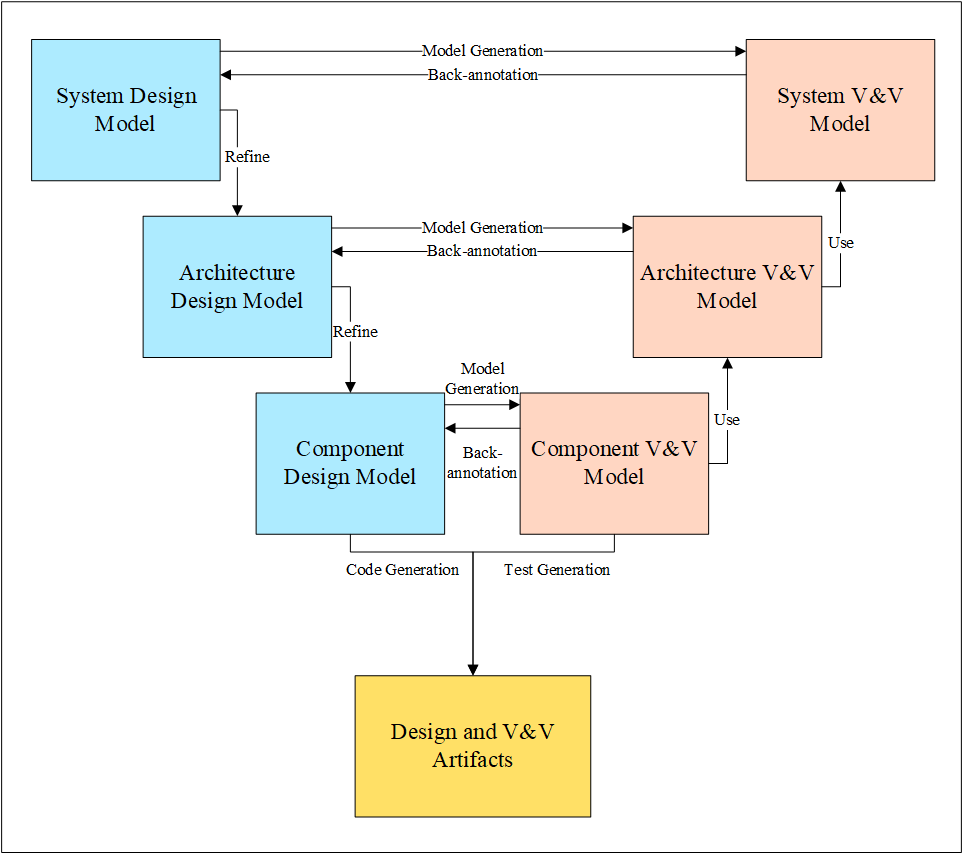
\includegraphics[width=100mm, keepaspectratio]{figures/yModel.png}
	\caption{The schematic description of the Y-Model}
	\label{fig:yModel}
\end{figure}

The process of deriving design artifacts is called \textit{model transformation}.
\begin{definition}[Model Transformation]
	Model transformation is the process of generating the target model from the source model. This process is described by by a transformation definition consisting of transformation rules, and a transformation tool that executes them. A transformation rule is the mapping of elements of the source model to the elements of the target model. \cite{ModelTransformation}
\end{definition}

Model transformations can be categorized based on the types of the source and target models: model-to-model (M2M), model-to-text (M2T), text-to-model (T2M) and text-to-text (T2T). These categories fundamentally define the tools required and usable for handling the different models.

There are also two important factors to consider when designing a model transformation: 
\begin{itemize}
	\item \textit{Consistency}: the same structure or behavior is described by the source and the target models (in their respective domains).
	\item \textit{Traceability}: the images of the original elements of the source model can be traced back to the original elements, from which they were generated.
\end{itemize}

%----------------------------------------------------------------------------
\section{Formal verification of systems} \label{section_background_FORM}
%----------------------------------------------------------------------------

Formal verification is the act of comparing the design model of a given system against certain requirements formulated by the stakeholders. This process requires mathematically precise design models and requirement specifications, but guarantees mathematical precision in its result as a proof of correctness or counterexample of the correct behavior.

\textit{Model checking} \cite{ModelCheckingClarkeGrumberg} is an automatic formal verification technique for a finite-state model of a system, which explores the state space of the given model soundly and often exhaustively. This results in a complete analysis of the behavior of the given system unlike in case of simulation or testing, which can only sample it.
The \textit{model checker} takes the formal model of the system and the formal requirement (a formula usually given in some kind of mathematical logic, which has to be satisfied by the system)  as an input, and returns the result of the evaluation often with a witness proving the result (see Figure \ref{fig:modelChecker}).
\begin{figure}[!ht]
	\centering
	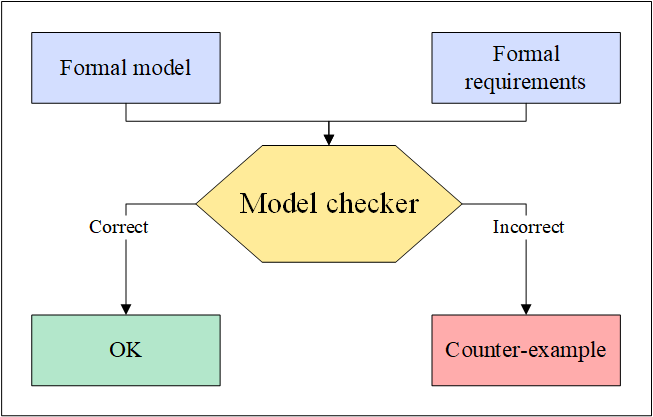
\includegraphics[width=70mm, keepaspectratio]{figures/modelChecker.png}
	\caption{The schematic description of the model checker}
	\label{fig:modelChecker}
\end{figure}

As the formal verification of the correct behavior is often a requirement against critical systems, the ability to transform the design model of the system into other models - in this case a verification model - proves to be a particularly useful quality. The precise formal analysis of these models either confirms the correctness of the given model, or provides example traces where the model does not meet the requirements. These faults can then be back-annotated to the high-level models, i.e. the tool can automatically identify the faulty section of the original model. This enables the system designer to make corrections, even in the early phases of the development process \cite{RoadToModelTransf}.

%----------------------------------------------------------------------------
\section{Formalisms for modeling behavior} \label{section_background_behaviorModeling}
%----------------------------------------------------------------------------

Different kinds of behavioral models grasp different aspects of the modeled system. \textit{State-based models} focus on the current state of the system and the change of states in response to the events of its environment. The process of this change is secondary, and these models consider these so-called transitions atomic and instantaneous. Examples of this kind of modeling include UML State Machines \cite{UMLStandard251} or statecharts \cite{HarelStatechart87}. On the other hand, \textit{process models} focus on the series of actions a system takes in order to achieve its goal, and these actions possess a temporal extent. Examples of this kind of modeling include UML Activity Diagrams \cite{UMLStandard251}, but the control flows of programs implemented in the popular imperative programming languages (e.g. C/C++, Java) are usually also process models. As these modeling languages often do not have precise semantics, it is common practice to define it by means of model transformations to formal models (denotational semantics). Several general-purpose imperative programming languages and process models used for their visualization can be easily transformed into Turing machines and many state-based models -- such as statecharts -- correspond well to finite-state machines.

One of the most important questions in the verification of computer programs is the ability to decide the termination of the given program -- known as the \textit{halting problem}. This is necessary, as to prove its correctness, the model checker analyzes the \textit{reachability} of certain states, for which it must traverse each possible execution of the given program. For Turing-complete models, the reachability of a given state is equivalent with the halting problem, and it is proven in \cite{Turing1936} that in general (i.e. for Turing machines), it is not possible to decide the termination for all program-input pairs. However, for finite-state machines, the problem is solvable \cite{Minsky:1967}. For this reason, it might be beneficial to restrict the system model to a finite-state machine for the sake of formal verifiability, especially in case of safety-critical systems, even if it possesses less expressive power than other types of automata. 
%Vince: senki földje a kettő között? (ebben a szakdogában nem)

According to automata theory, finite-state machines can be considered a specialized form of pushdown automata, which, in turn, are a specialized kind of Turing machines (see Figure \ref{fig:automataTheory}). This, through the associations made earlier in this section, provides us with an excellent basis of comparison for different types of system models.

\begin{figure}[!ht]
	\centering
	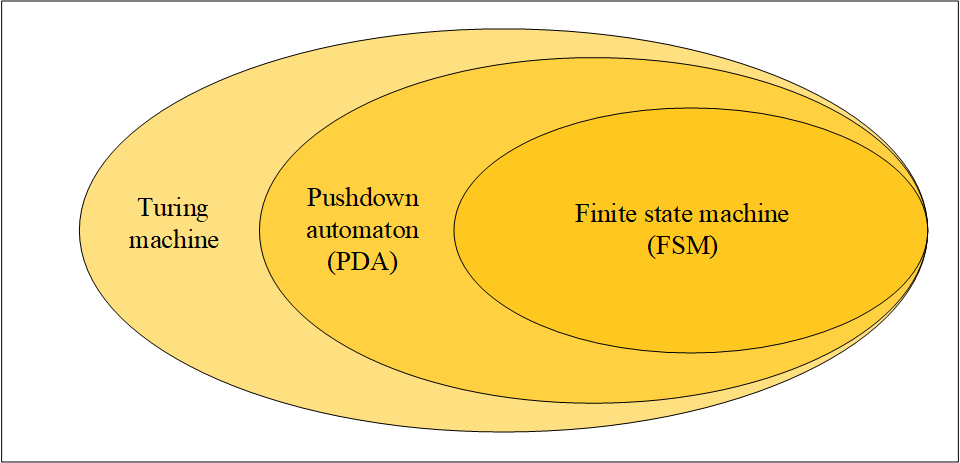
\includegraphics[width=100mm, keepaspectratio]{figures/automataTheory.png}
	\caption{Classes of automata}
	\label{fig:automataTheory}
\end{figure}

%----------------------------------------------------------------------------
\section{Statechart formalism} \label{section_background_statechart}
%----------------------------------------------------------------------------
Although in engineering the \textit{statechart} formalism is the more convenient way to describe reactive systems, the mathematical basis of this modeling language is the so-called \textit{finite-state machine}.

\begin{definition}[Finite-state Machine]
	A finite-state machine (FSM) is a model of computation to describe the behavior of a system in reaction to the events of its environment \cite{BaeStateMachine}. Mathematically, a finite-state machine is $M = (S, s_0, I, O, T)$  where:
	\begin{itemize}
		\item $S = \{s_0, s_1, s_2, \dots , s_n\}$ is a finite set of states,
		\item $s_0$ is the initial state, 
		\item $I = \{i_0, i_1, \dots , i_p\}$ is a finite set of input events, that are stimuli from the environment, 
		\item $O = \{o_0, o_1, \dots , o_q\}$ is a finite set of output events, that are stimuli for the environment,
		\item $T : (I \times S) \to (S \times O) $ is the transition function, that represent changes of states in response to input events and generating output events.
	\end{itemize}
	A possible sequence of steps can be described through a \textit{trace}. A trace is a finite sequence of alternating states and transitions beginning and ending in a state: $\varrho = s_0, t_0, s_1, \dots , t_{n-1}, s_n$, where $s_i \in S$ and $t_i \in T$.
	%$\varrho = s_0, i_0/o_0, s_1, \dots , i_p/o_q, s_n.$ 
	%$\varrho = ((i_0, s_0, s_1, o_0), (i_1, s_1, s_2, o_1), \dots , (i_p, s_{n-1}, s_n, o_q))$.
\end{definition}

The \textbf{\textit{statechart}} \cite{HarelStatechart87} formalism is a possible extension of this mathematical model with the following elements. Conforming to the UML Standard \cite{UMLStandard251}, it includes the following extensions to finite-state machines:	
\begin{itemize}
		\item States
		\begin{itemize}
			\item hierarchical states: states that themselves have a state space.
			\item concurrent regions: a state is active in each of the regions, which operate asynchronously.
			\item actions assigned to states (entry, exit, do): behaviors that happen when a state becomes, is, or stops being active.
		\end{itemize}
	\item Pseudo-states
		\begin{itemize}
			\item initial state: a state which is only active when the execution of the region starts.
			\item final state: a state which is only active when the execution of the region ends.
			\item history states (deep and shallow history): states that are active when the execution of a region starts, with the next state being where the execution of the region previously stopped.
		\end{itemize}
	\item Transitions
		\begin{itemize}
			\item given in the form: trigger [guard] / action, that determine the possible following states depending on the state of the system and the incoming events, also describing the reaction of the system during the change of states.
			\item complex transitions (fork-join, branching): for handling concurrency and decisions. 
		\end{itemize}
	\end{itemize}
The syntax of the possible actions is detailed in an \textit{action language}, which is different from tool to tool, along with some further extensions. The features of this action language determine whether the system model corresponds to an FSM or a more general type of automaton -- with the corresponding expressive and verification capabilities.

The action language designed in the following chapters has the goals of having a fairly high expressive power and supporting formal verification. According to the previous section, the compromise is to remain at the complexity of FSMs by only supporting high-level imperative programming constructs that possess at most the expressive power of that formalism.
%TODO PDA

%----------------------------------------------------------------------------
\section{Related Work} \label{section_background_comparison}
%----------------------------------------------------------------------------
To be able to determine the best-practices and dead-ends, we have to analyze the action languages of existing tools. We are going to use the definition of action provided in the UML Standard \cite{UMLStandard251}.
\begin{definition}[Action] \label{definition_action}
	An action is a fundamental unit of computational behavior specification. An action takes a set of inputs and produces a set of outputs. It may also modify the state of the system.
	
	It is important to note that the sets of inputs and outputs may also be empty.
\end{definition}

In the following sections, we are going to inspect various modeling tools, with special attention to their action languages, or, if not explicitly defined, their process-oriented reaction description capabilities.

\subsection{UML 2} \label{subsection_background_comparison_UML}
The Unified Modeling Language (UML) \cite{UMLStandard251} is a general-purpose graphical modeling language for the domain of software engineering. In recent years, it has become the standard way to visualize the design of software systems. Examples of UML diagrams include use-case diagrams, class diagrams, sequence diagrams, activity diagrams, state machines, etc.

According to the UML Standard \cite{UMLStandard251}, the means of describing actions is through Actions (with capital A). Actions are defined as in Definition \ref{definition_action}. Actions (ActivityNodes) are always contained in Behaviors (Activities or Interactions), that define the context of the execution of the Action. The execution of an action represents some transformation or processing in the modeled system. The standard defines several types of actions (specializations of ActivityNode), for instance Invocation Actions, Object Actions, Link Actions, Structural Fearute Actions, Variable Actions, Accept Event Actions. One special kind of Actions are Structured Actions (StructuredActivityNodes), which are not only Actions, but also ActivityGroups. This means, that Structured Actions can contain Activities (a graph of ActivityNodes and ActivityEdges defining the control and data flow of a Behavior) and Variables. Besides that, another construct called Expansion Region is available, which has an input collection (a given set of input data for the region), and executes the contained StructuredActivityNode for each of the elements of the input collection, each time providing the current element as input data.

In addition to the Actions defined in the standard, OpaqueActions are also available for modeling actions. OpaqueActions are Actions, for which the specification may be given in a textual syntax other than UML. It consists of body and language strings. If multiple of those elements are available, the standard does not determine how the choice is made. This is one example of syntactic and semantic variation points and results in the modeling of arbitrary actions, making the language extremely versatile.

Variability of syntax and semantics is deliberately included in the modeling language, as discussed in \cite{VariabilityInModelingLanguages}. This promotes the communication of engineers and the visualization of systems, but results in an incomplete definition of the language. Therefore, UML models in general are not suitable for code generation or formal verification. 

\begin{figure}[!ht]
	\centering
	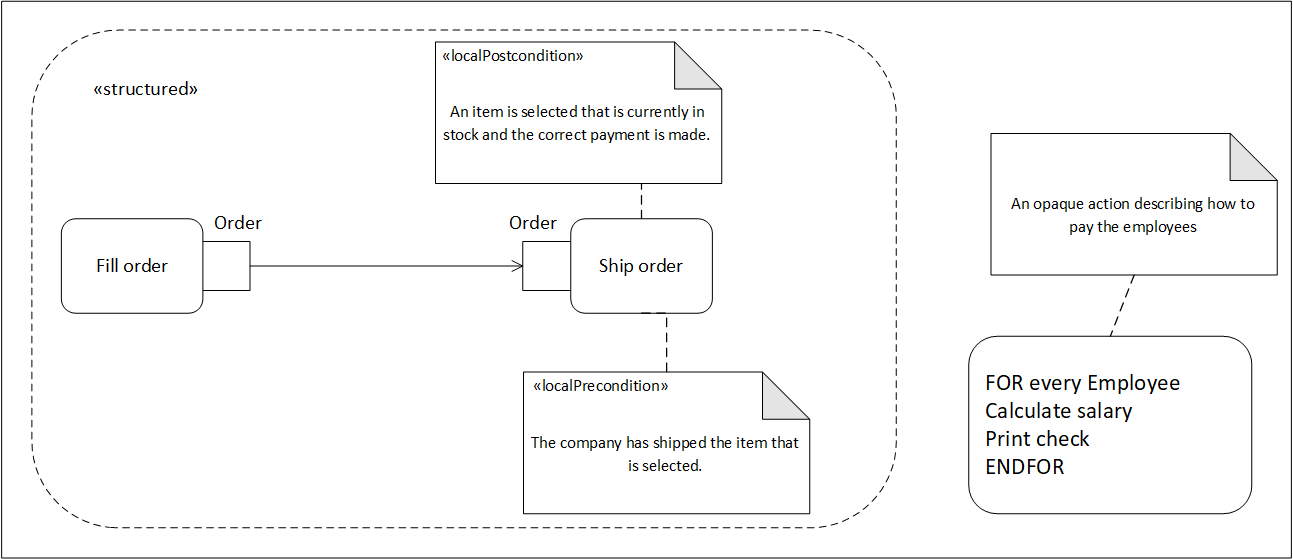
\includegraphics[width=150mm, keepaspectratio]{figures/UMLAction.png}
	\caption{A Structured Activity (left) and an Opaque Action (right) according to UML 2.5.1}
	\label{fig:UMLAction}
\end{figure}

\subsection{fUML and Alf} \label{subsection_background_comparison_fUMLAlf}
Foundational UML (fUML) \cite{fUMLStandard} is a computationally complete subset of the UML 2 standard with a precise definition of the operational semantics of that subset and serving as a foundation for higher-level UML modeling concepts. It defines a basic and general virtual machine for UML, enabling the transformation of the models into executable forms for verification, integration and deployment. It attempts to maintain a degree of genericity in order to support various execution paradigms, environments and underlying data structures. This is achieved by leaving certain key semantic elements (e.g. time, concurrency, inter-object communication) unconstrained and explicitly defining semantic variation points (e.g. event dispatch scheduling, polymorphic operation dispatching). The majority of the standard is defined by excluding elements of the UML2 standard.
%TODO: mention xUML and Scrall

fUML offers similar mechanisms for describing actions as UML, applying several restrictions to the elements of the latter. For instance, custom constraints are not supported in fUML, therefore, local pre- and postconditions are not supported either. Redundant elements are also excluded from the standard, like ActionInputPins and ValuePins, as they can be represented using object flow. Variable Actions are also excluded, as Variables are not supported in fUML -- they too can be represented using object flow. Structured Actions are still supported with the exclusion of Variables and Sequence Nodes (that would execute a sequence of ExecutableNodes in order), similarly to Expansion Regions with no exclusions. However, Opaque Actions are excluded, as, being opaque, they cannot be executed.

An alternative to this is the Action Language for Foundational UML (Alf) \cite{AlfStandard}. It is a textual surface representation for UML modeling elements, mapping a textual concrete syntax to the abstract syntax of the fUML standard. The main focus of Alf is to be an action language, but it also provides concrete syntax for modeling structural elements of fUML. It possesses a naming system based on UML, an implicit type system for activities and also the expressivity of OCL \cite{OCLStandard} with a C-like syntax, also allowing the UML textual syntax whenever it exists (e.g. type declaration of variables after the name and a colon, as opposed to before the name of the variable). 

To examine the formal verification capabilities residing in fUML and/or Alf, it suffices to analyze one or the other, as Alf is directly mapped to the fUML abstract syntax. In comparison to UML2, the majority of semantic variation points are either precisely defined or eliminated, thus, models created according to these standards are transformable into executable ones, enabling verification. Nonetheless, due to the Turing completeness of fUML, the termination of the possible algorithms cannot be guaranteed - the language is \textit{undecidable}. Hence, the correctness of the models with regard to the requirements cannot be formally verified in all cases by a model checker.

\begin{figure}[H]
	\centering
	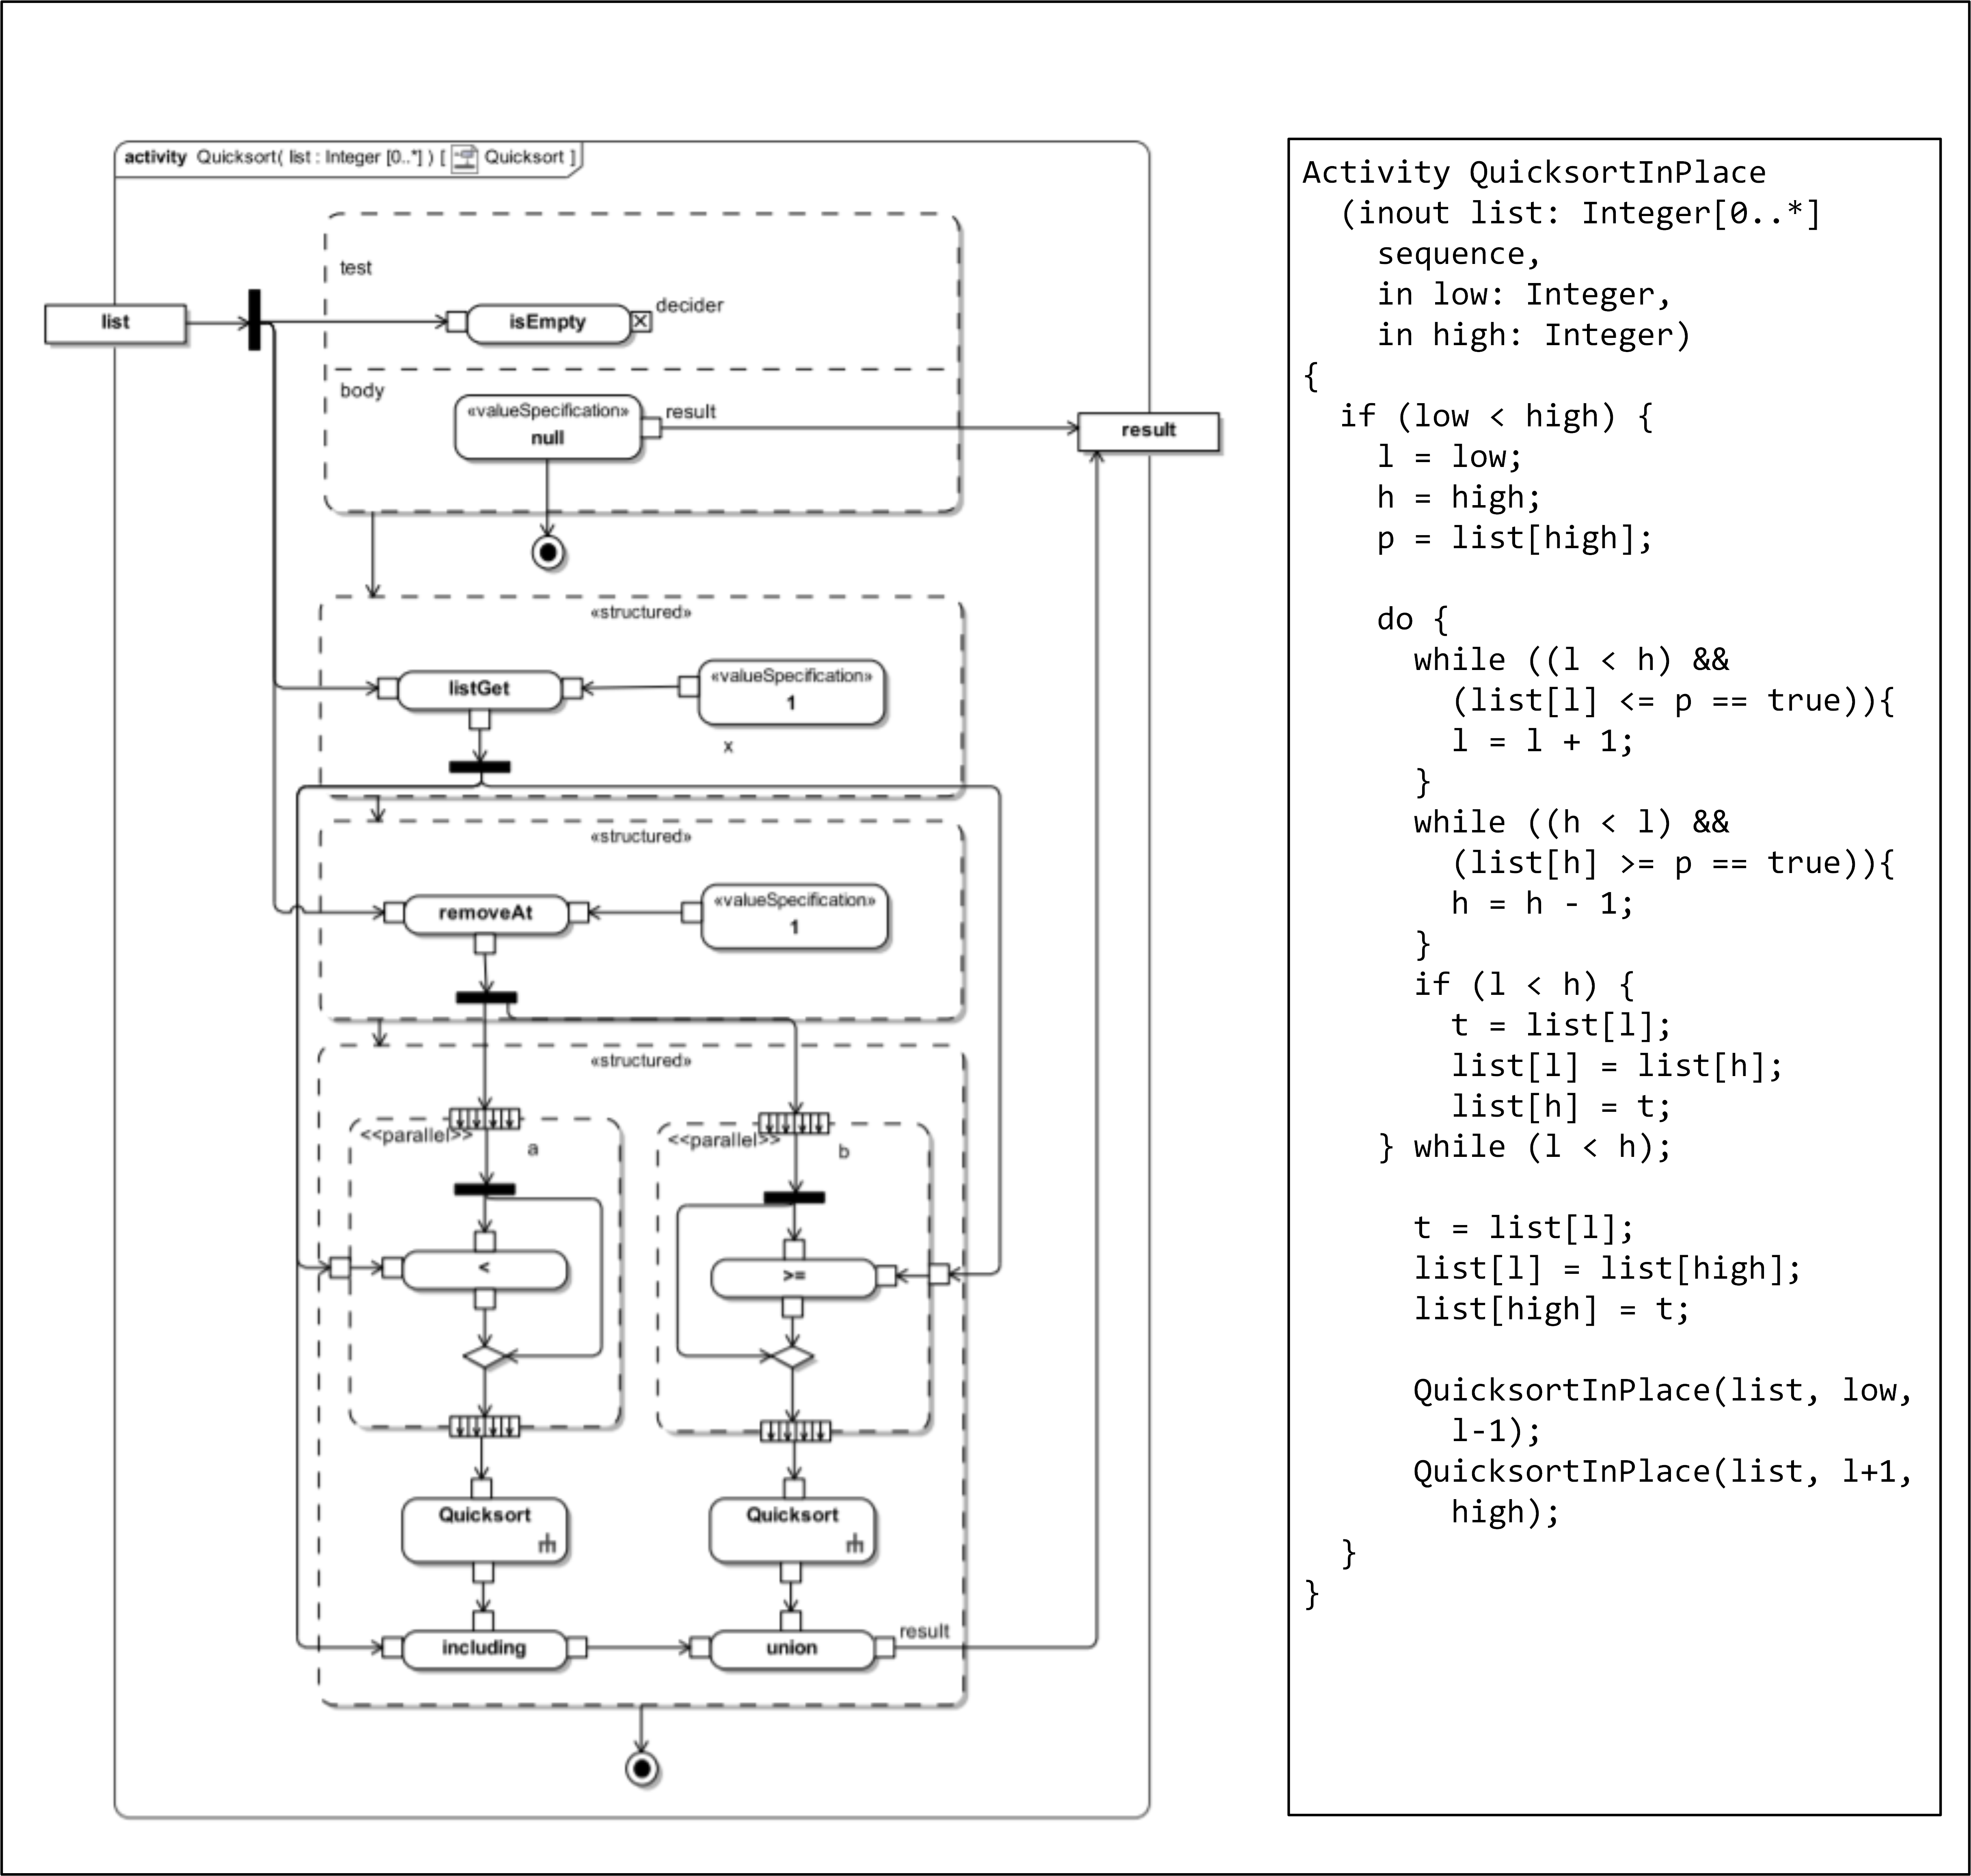
\includegraphics[width=140mm, keepaspectratio]{figures/AlfQuicksort.png}
	\caption{Quicksort algorithm using fUML (left) and Alf (right) from Appendix B of \cite{AlfStandard}}
	\label{fig:AlfQuicksort}
\end{figure}

\subsection{Yakindu Statechart Tools} \label{subsection_background_comparison_Yakindu}
YAKINDU Statechart Tools is a modular toolkit for the development and analysis of reactive, event-driven embedded systems using the statechart formalism, already discussed in Section \ref{section_background_statechart}. It combines graphical and textual syntax for the modeling of systems, and, among others, supports the simulation and source code generation for the designed statecharts. Yakindu consists of the following features for dealing with statecharts: statechart diagram editor, statechart simulator, code generators, generator projects for custom model transformations, validator, unit testing framework, C language integration and a debugger.

In Yakindu statecharts, transitions may have reactions in the form \textit{trigger [guard] / effect}. Also, states may possess entry effects and exit effects in the form \textit{entry / effect} and \textit{exit / effect} respectively, and local reactions containing effects, such as \textit{every 1s [guard] / effect}. The elements permitted in the specification of effects are called actions, and together, they constitute the action language of Yakindu. 
An effect contains zero, one or more actions, separated with semicolons. Normally actions are statements, which are either assignments, event raisings, or operation calls. Assignments in Yakindu assign a given value to a given variable, possibly evaluating an arithmetic or logical expression meanwhile. Event raising takes place using the \textit{raise} keyword and the name of the event to be raised. Operations are functions declared in a C header (.h) file and implemented outside of Yakindu, which is then available to be called from a statechart using an operation call. An operation is called similarly to other programming languages, using the name of the operation and passing the actual arguments in parentheses.

Regarding the possibilities of the verification of Yakindu statecharts, the editor offers some verification capabilities in the form of a simulator and a unit testing framework. However, these tools are able to analyze the behavior of a certain system model through manual sampling only. Formal verification capabilities are currently not available in the tool, although it is possible by transforming Yakindu models to models verifiable by other tools, such as UPPAAL -- similarly to the workflow of the Gamma Framework. Naturally, operation calls can only be formally verified if the target language can be formally verified, which is in general not possible for the C language.

\begin{figure}[ht]
	\centering
	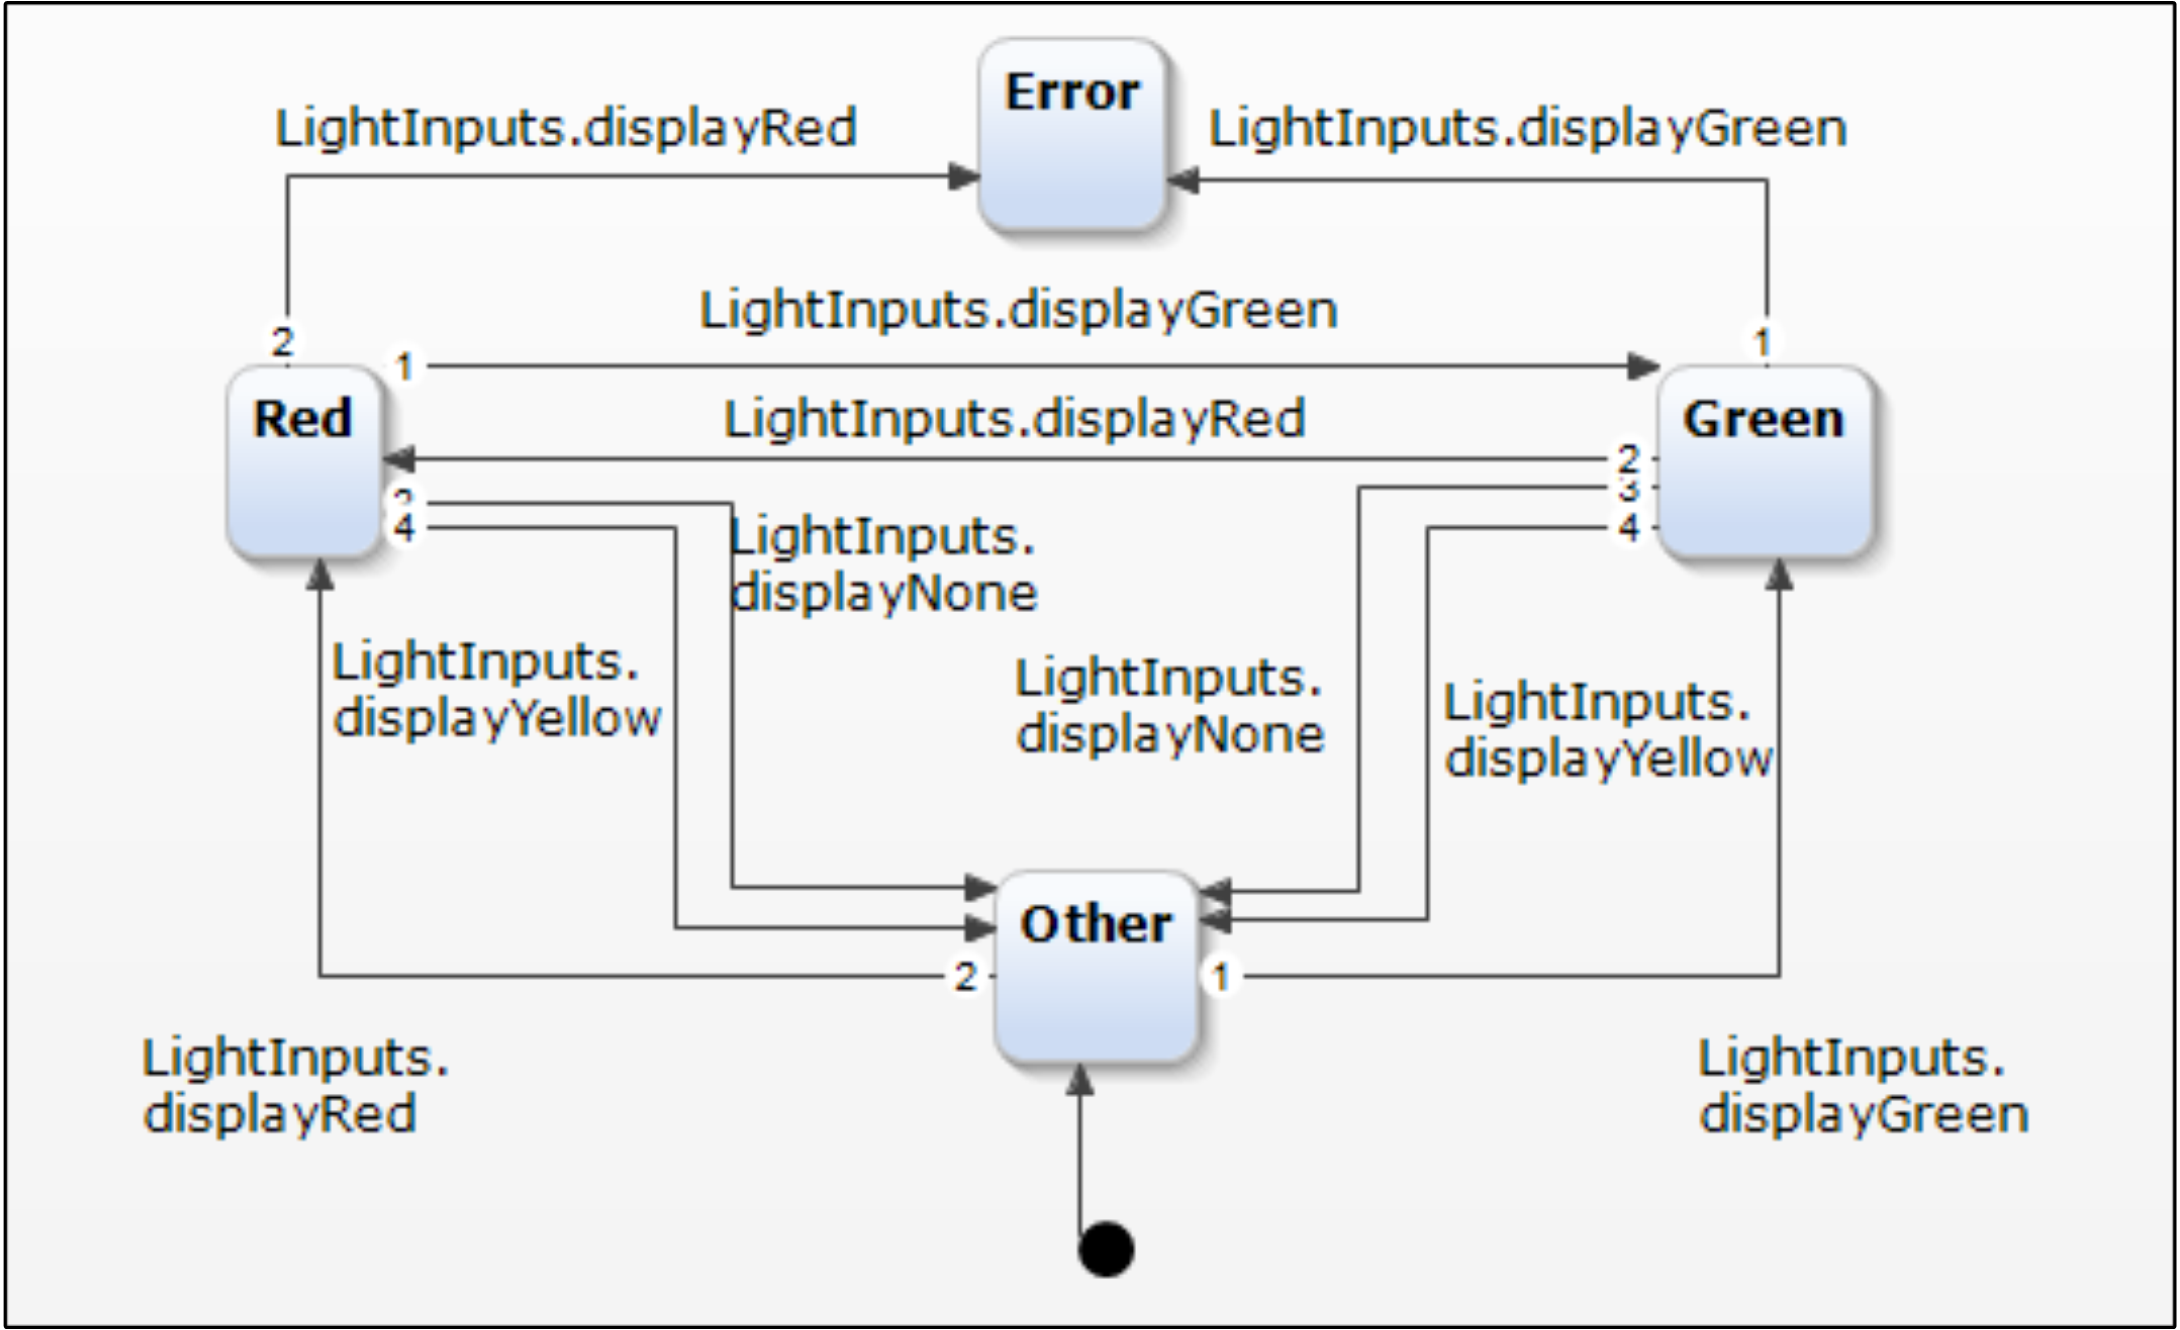
\includegraphics[width=100mm, keepaspectratio]{figures/YakinduAction.png}
	\caption{Yakindu statechart containing \textit{raise event} actions}
	\label{fig:YakinduExample}
\end{figure}

\subsection{UPPAAL} \label{subsection_background_comparison_UPPAAL}
UPPAAL is a tool for modeling, simulation and verification of real-time systems \cite{UPPAALTutorial, UPPAALPresentAndFuture}. UPPAAL uses the timed automata formalism described in \cite{TimedAutomataDef}, extended with integer variables, structured data types, user defined functions and channel synchronisation. The main focus of the tool is the model-checking of systems modeled as networks of timed automata.

For the complete description of the capabilities of the UPPAAL tool, we refer the reader to \cite{UPPAALTutorial}, here only follows a short summary of the referred paper for clarity of the following paragrahs. In UPPAAL, the root element is the Network of Timed Automata, which contains Templates. Templates are models of (extended) timed automata, which can be instantiated, then called Processes. Templates have parameters that can be bound to values during instantiation, locations (possible "situations" of the automaton), and edges (conforming to the semantics of transitions in standard timed automata). UPPAAL also allows the use of variables and clocks, and the 3-tuple (location, variables, clocks) defines the state of a Process. Asynchronous automata can interact by using synchronization channels. Locations may contain invariants -- Boolean-evaluated expressions that must always hold when the automaton is in the given location. Edges may contain channel synchronizations, guards, updates and selection expressions. From UPPAAL 4.0, user-defined functions -- defined using a specialized subset of the C language -- are also allowed.
%TODO: think about what languages are not an extended subset of C

As we can see, there are no explicitly defined actions in UPPAAL, therefore, we consider the process of the reaction of the system an action, based on Definition \ref{definition_action}. This is met by updates and selection expressions found on edges. Updates are expressions with side effects that change the state of the system, such as assignments. Selection expressions non-deterministically bind a given identifier to a value in a given range that is valid in the scope of the given edge -- basically being a special kind of local variables. It is important to note, that user-defined functions may appear as part of these expressions. For functions without side effects, the evaluation is equivalent to the evaluation of expressions. For functions with side effects, however, the evaluation of the effect could become a more complex task.

UPPAAL is a tool for the formal verification of the above mentioned systems, so the ability of verification of the modeled systems follows naturally from the nature of the tool. The evaluation of edges is atomic, which is extremely important in case of user-defined functions: the syntax permits many constructs from C (except e.g. pointers) extended with timed automata-specific elements. However, these elements are defined in a way that ensures the termination of these functions -- e.g. allowing only foreach-loops, or bounded integers. Naturally, this might have an effect on the performance, but does not prevent verifiability in general.
%TODO: can UPPAAL get into livelocks through functions?

An example of an UPPAAL automaton can be seen on Figure \ref{fig:UPPAALGossipingGirls}, based on an example in \cite{UPPAALTutorial}. It aims to model the behavior of 'girls' in the following example: let there be \textit{n} girls, each aiming to share their private secrets with all the others. Any girl can call anyone, and after a conversation, both know all the secrets of both of them. The question is, how many calls are necessary in total, so that in the end each of the girls knows everything. Based on this description, the girls in the model can demontrate two different behaviors: either call another girl (represented by sending a channel synchronization), put their secrets in a common temp variable, then copy the 'merged' secrets when the other one also put their secrets in, or wait for a call (by waiting for a channel synchronization), then merge their secrets with those of the other one, and copy the secrets for themselves.

\begin{figure}[!ht]
	\centering
	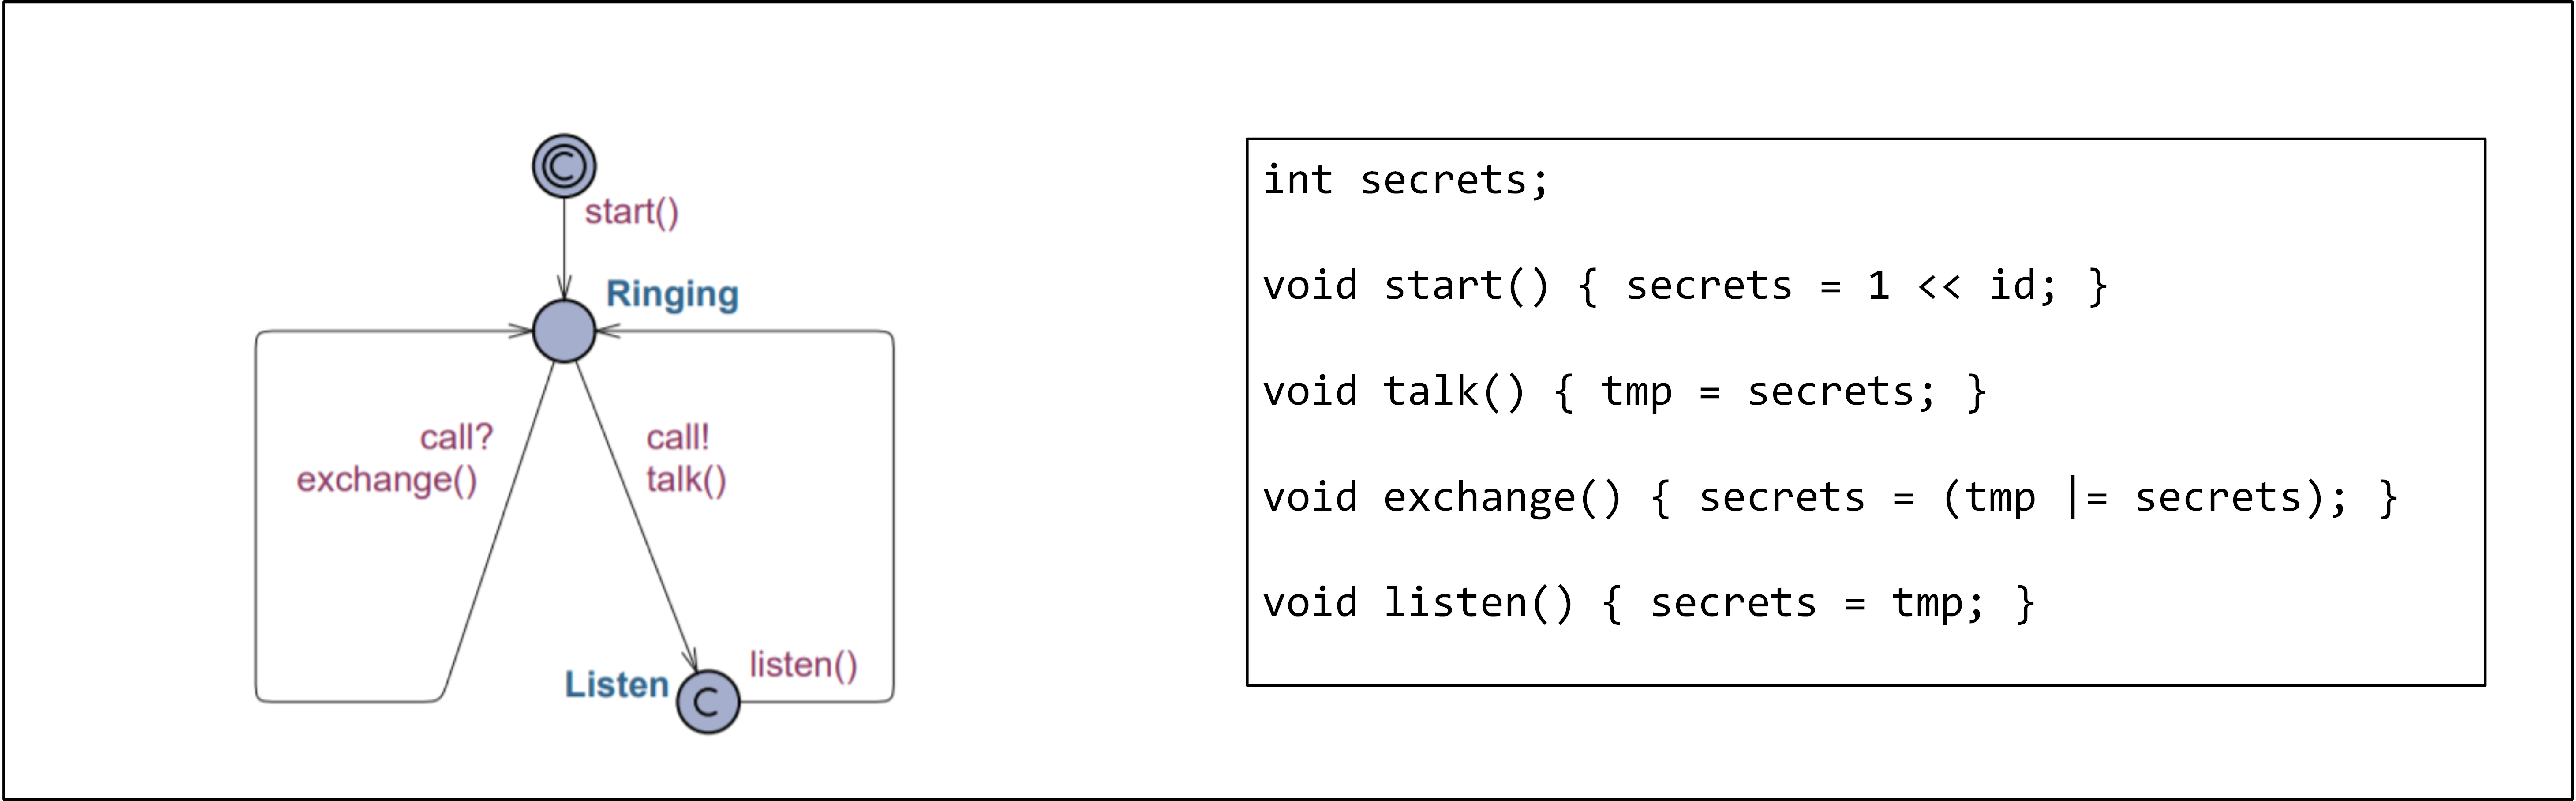
\includegraphics[width=150mm, keepaspectratio]{figures/UPPAALGossipingGirls.png}
	\caption{Template automaton of the Gossiping Girls problem along with the corresponding function definitions}
	\label{fig:UPPAALGossipingGirls}
\end{figure}

One important thing to note about the timed automaton formalism of UPPAAL is the fact that it results in models that are difficult to implement, its constructs being abstractions of real-world behaviors -- e.g. channel syncronizations or the bitshift and bitwise OR operators in the example. Therefore, it is impractical to model complex systems in UPPAAL. A viable alternative is transforming existing system models to UPPAAL timed automata for verification, which is exactly what the Gamma Statechart Composition Framework does.

%----------------------------------------------------------------------------
\section{Target Technologies} \label{section_background_target}
%----------------------------------------------------------------------------

\subsection{Gamma Statechart Composition Framework} \label{subsection_background_target_gamma}
The Gamma Statechart Composition Framework \cite{GammaVince2018} is a tool that facilitates the design, verification, validation and code generation for component-based reactive systems. It defines its own, domain specific statechart composition language for assembling the system model from its components modeled using the statechart formalism. It aims to fill the gap between UML tools, which are used for visualization of the composition of systems, and the various statechart modeling tools, such as Yakindu, that enable system designers the modeling of reactive system components.

The Gamma Framework offers the Gamma Composition language (GCL) for the modeling of components, interfaces, ports and communication channels. Components can be either composite components -- which define a composition of components by instantiating other components, binding their ports to the ports of the composite component and defining communication channels between components -- or statecharts, which are the basic building blocks defined through the Gamma Statechart Language (GSL).

In GCL, the components communicate through ports, through which they send or receive certain predefined signals, called events. Events are declared on interfaces, which are realized by ports. They can also be parametrized, passing additional data along with the basic signal. This functionality is implemented using variables -- boolean-type for the events, and the appropriate type(s) for the parameter(s) --, that can be accessed on both ends of the channel. Channels are always one-directional, the sending and the receiving end are specified at the interface realizations.
There are also special events, called timeout events, which fire when a previously set timeout variable signals at the end of the specified time interval. 

The GSL can be used to define statecharts of the Gamma Framework. This formalism provides a textual representation for the modeling of statecharts, unlike the ordinary graphical representation. Gamma Statecharts can be parametrized, and can also have ports -- interfaces which they realize as required or provided. They may have variables (which are visible in the scope of the statechart), timeout variables, transitions and a region. The region contains the states, between which the transitions can run. Transitions may have triggers (the events to which the transitions fire), guards (additional conditions for the possibility of the firing of a transition) and several actions (reaction specifications of the system). States always have names and may contain invariants, entry and exit actions, and also additional regions.

The framework also supports executable code generation for the modeled systems. Gamma can generate source code not only for the modeled statecharts, but also for the composition code on top of these components, due to the precisely defined compositional semantics. Also, it allows the integration of external code generators. The currently supported target language is Java.

The numerous features of Gamma also include the application of hidden formal methods for the verification of the modeled systems. It is especially useful combined with the high-level user interface with elements designed for efficient model checking. For comparison, the modeling of systems in other tools also offering formal verification is often difficult, due to the low-level modeling elements these tools offer.

Gamma also allows the integration of third-party statechart modeling tools and model-checkers, currently containing an implementation for the integration of Yakindu Statechart Tools discussed in Section \ref{subsection_background_comparison_Yakindu}, UPPAAL discussed in Section \ref{subsection_background_comparison_UPPAAL}, and the transformation for the Theta verification framework (Section \ref{subsection_background_target_theta}) is under development. Back-annotation of the generated models is also supported for these tools.

While there are tools with similar goals, the distinctive quality of Gamma is supporting all the above mentioned features by defining an intermediate model that allows the integration of third-party tools with different target functionalities in the domain of critical systems.

An example of a Gamma statechart can be seen on Figure \ref{fig:gammaExample}.

\begin{figure}[!ht]
	\centering
	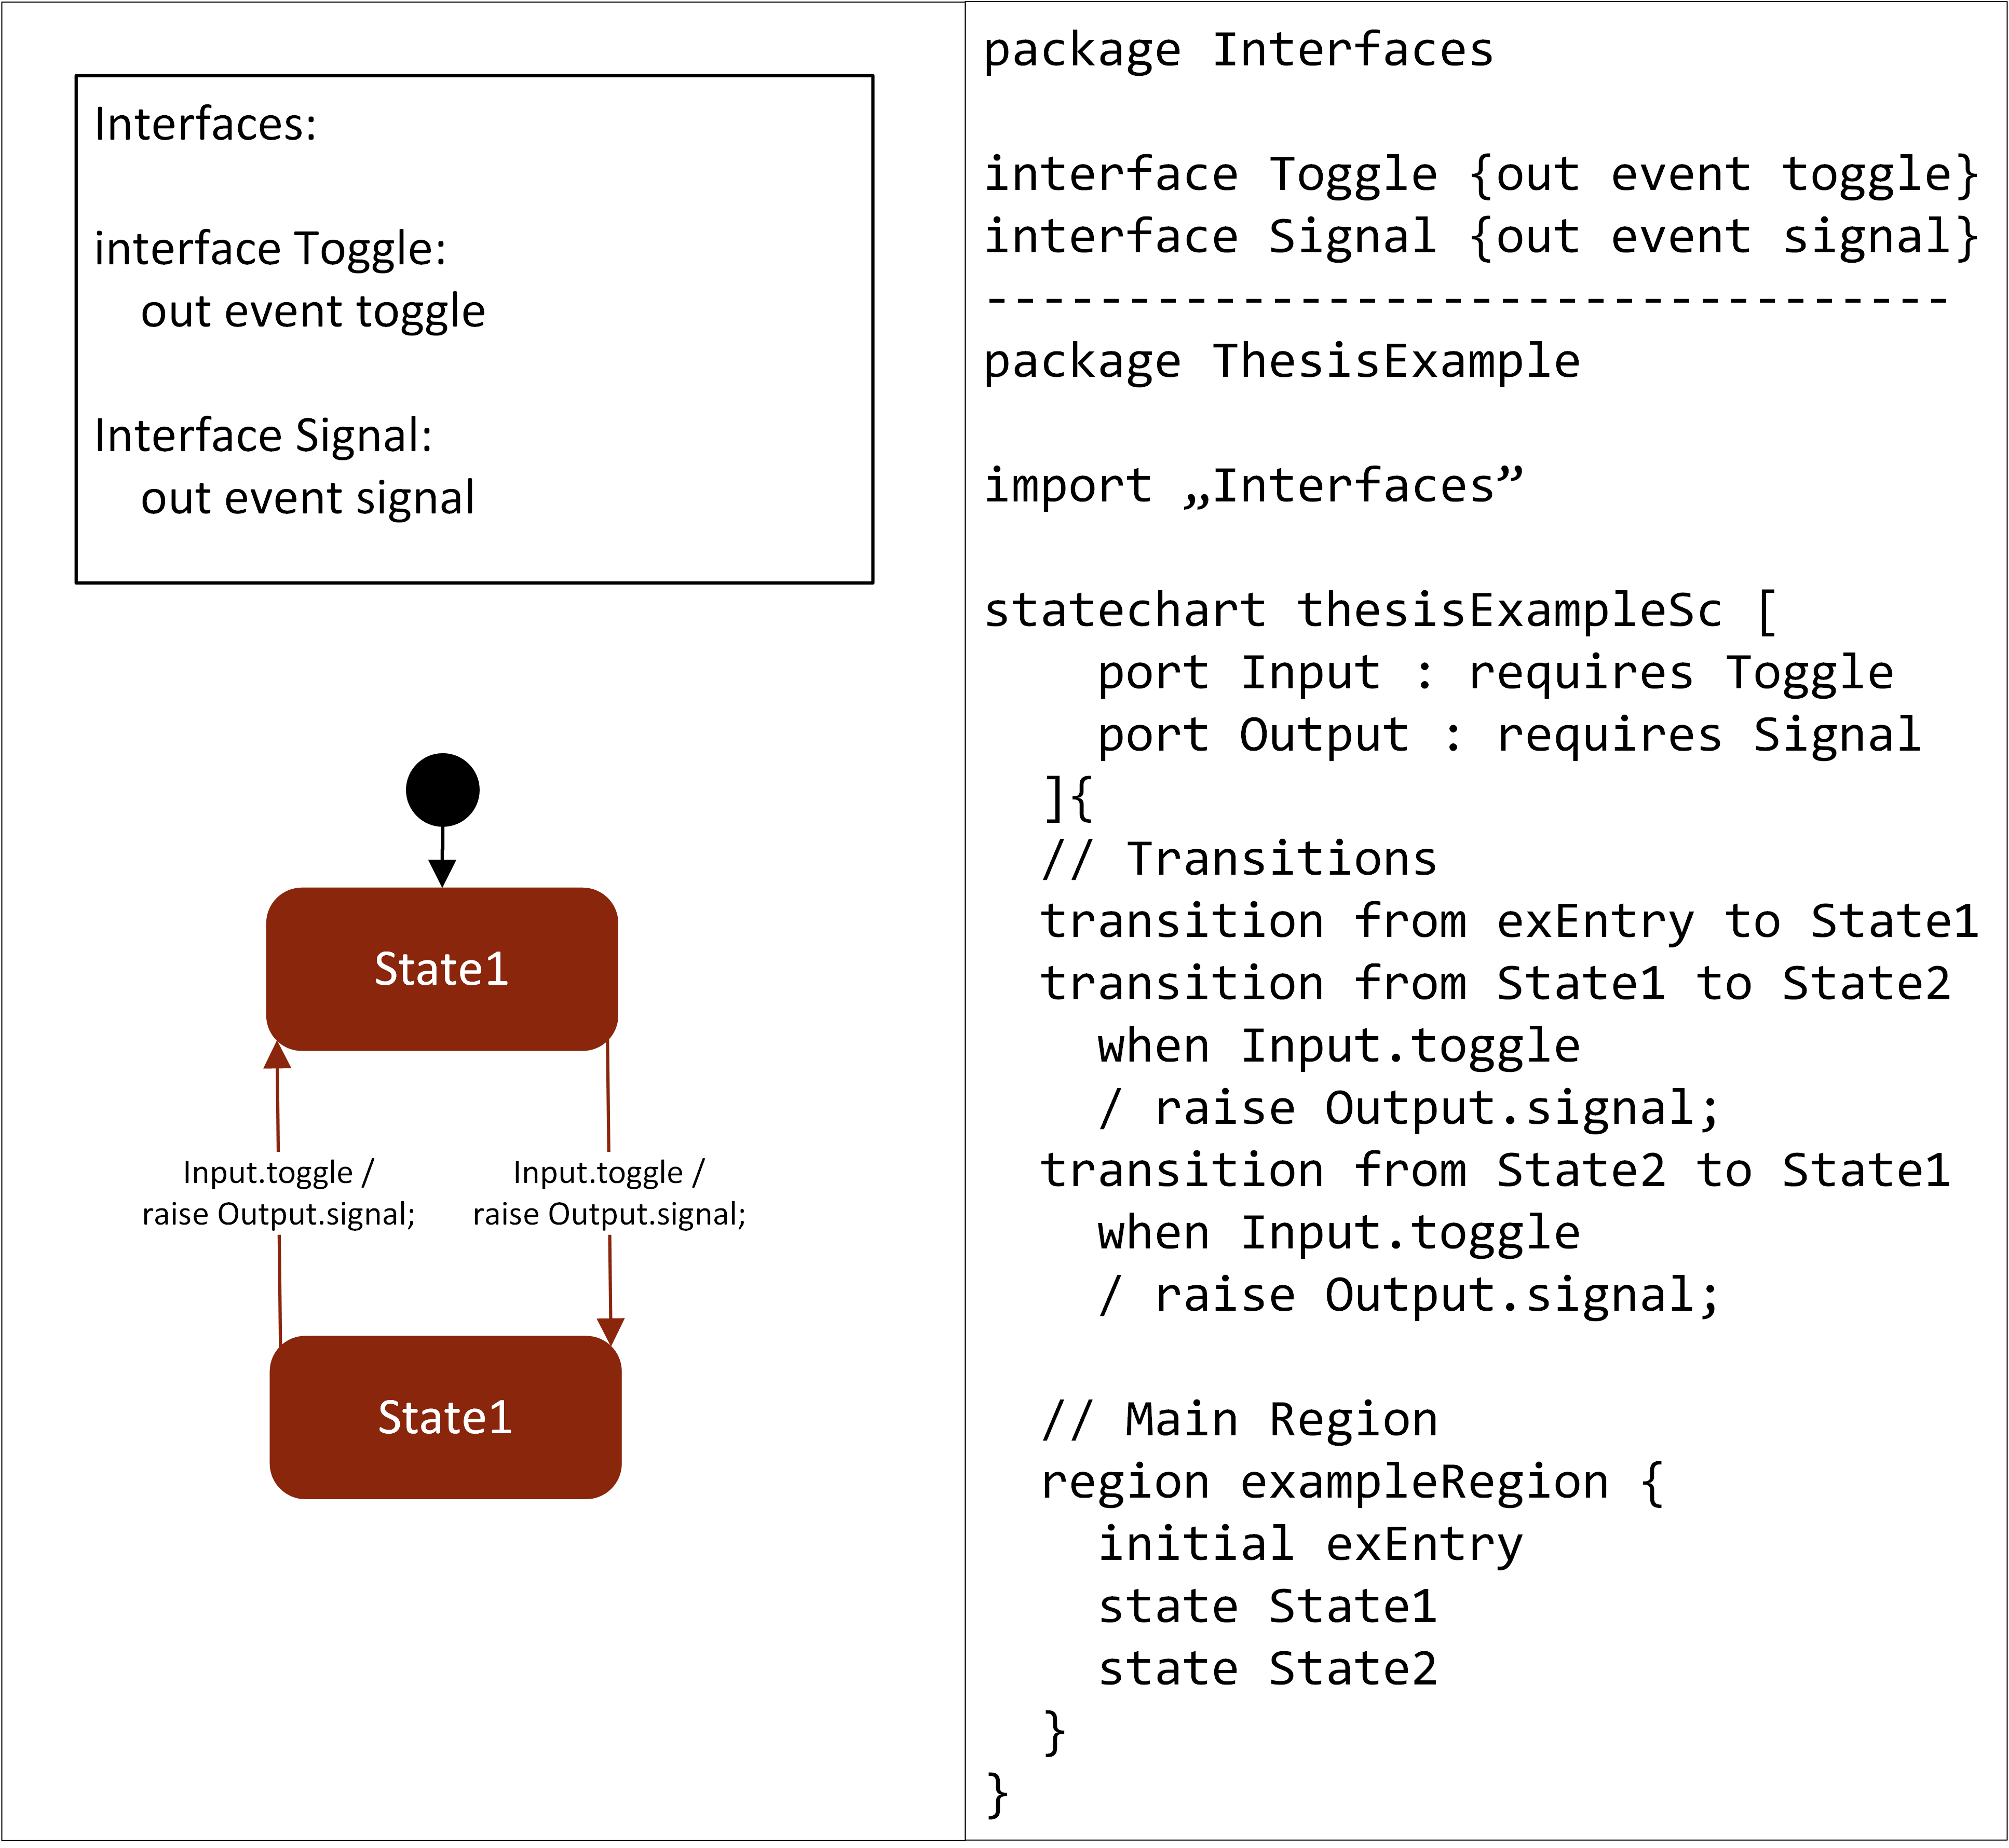
\includegraphics[width=90mm, keepaspectratio]{figures/gammaExample.png}
	\caption{A Gamma statechart (right) and the corresponding visual representation (left)}
	\label{fig:gammaExample}
\end{figure}

\newpage
\subsection{Theta} \label{subsection_background_target_theta}
The Theta Framework \cite{ThetaToolPaper} is a model checking framework that supports the development and evaluation of abstraction refinement-based algorithms, which are, in turn, useful for the reachability analysis of different formalisms. It aims to solve the problem of having to use different model checking tools for different analysis algorithm and modeling formalism pairings, by offering a generic solution, which is freely extensible. The rationale behind this solution is the fact that no single configuration of formalisms and analysis algorithms can verify all models, and the execution times also vary greatly.

The framework itself is generic, modular and configurable, which allows researchers to implement, evaluate and compare new components and combinations. The genericity and modularity allow for new components to be freely implemented, and the configurability results in the possibility to use and evaluate any of the implemented combinations. 

The main parts of the framework are the formalism and language-front ends, the analysis back-end and the SMT solver interface. The first two can be extended and configured by the user, and the latter can be used by the analysis components for communication. In addition, Theta contains three concrete, built-in tools for the verification of transition systems, control flow automata, and timed automata. 

%Symbolic transition system formalism: 
%	STSs: consists of states and transitions and the local properties of states are represented as labels. The states are represented as state variables, labels can be parametrized and update functions are defined (for which if the defined constraint is evaluated to true, corresponding update mapping is applied). They provide a finite representation to model the state behavior of systems with possibly infinite state spaces. They treat data symbolically
%	They differ from FSMs, as: sets of states and transitions may be infinite + no initial and final states are defined.
%	Very LL
%	Based on SMTs: 
%		Generalization of SAT for formulas in more advanced theories than propositional logic.
%		SMT solvers genralize the concept of SAT solvers.

%Theta STS: consists of an initial expression, a transition relation expression and a property expression. 
